\documentclass{beamer}
\usetheme{Boadilla}
\setbeamertemplate{navigation symbols}{}
\setbeamercovered{invisible}
\useinnertheme{rounded}

%Palatino + AMS Euler
\usepackage[euler-digits,euler-hat-accent]{eulervm}
\usefonttheme{serif}
\usepackage{fontspec}
%\setmainfont{TeX Gyre Pagella}


\usepackage{tikz}
\usepackage{tikzscale}
\usetikzlibrary{shapes,arrows.meta}
\usetikzlibrary{positioning}
\usetikzlibrary{math}
\usetikzlibrary{external}
\tikzexternalize[optimize=false,prefix=tikz/]
\usepackage{amssymb}
\usepackage{nicefrac}
\usepackage{amsmath}
\usepackage{siunitx}
\usepackage{mathtools}
\usepackage{booktabs}
\usepackage{graphicx}
\sisetup{range-phrase=...}
\usepackage{pgfgantt}
\usepackage{soul}
\usepackage{pgfplots}
\pgfplotsset{compat=newest}
\usepgfplotslibrary{fillbetween}
\usepgfplotslibrary{groupplots}
\usepackage{listings}
\usepackage{tabularx}
\usepackage{subfig}

\definecolor{juasblue}{rgb}{0,0.5411,0.7647}
\definecolor{juasgrey}{rgb}{0.49,0.698,0.761}
\graphicspath{ {./img/}}

\title[Practical Days - RF]{CERN practical days - RF}
\subtitle{09:00} 
\author[Heine, Noll]{Ruben Heine \and Marvin Noll}
\date[\today]{14.03.2022}

\makeatletter
\colorlet{beamer@blendedblue}{juasblue}
\makeatother

\begin{document}
\begin{frame}[plain]
  \titlepage
\end{frame}

\begin{frame}{Outline}
    \tableofcontents
\end{frame}

\section{Forenoon Session}
\subsection{Band Pass Filter}
\begin{frame}[t,fragile]{Band Pass Filter (1) - Transmission $S_{12}$, $S_{21}$}
\begin{figure}
  \centering
  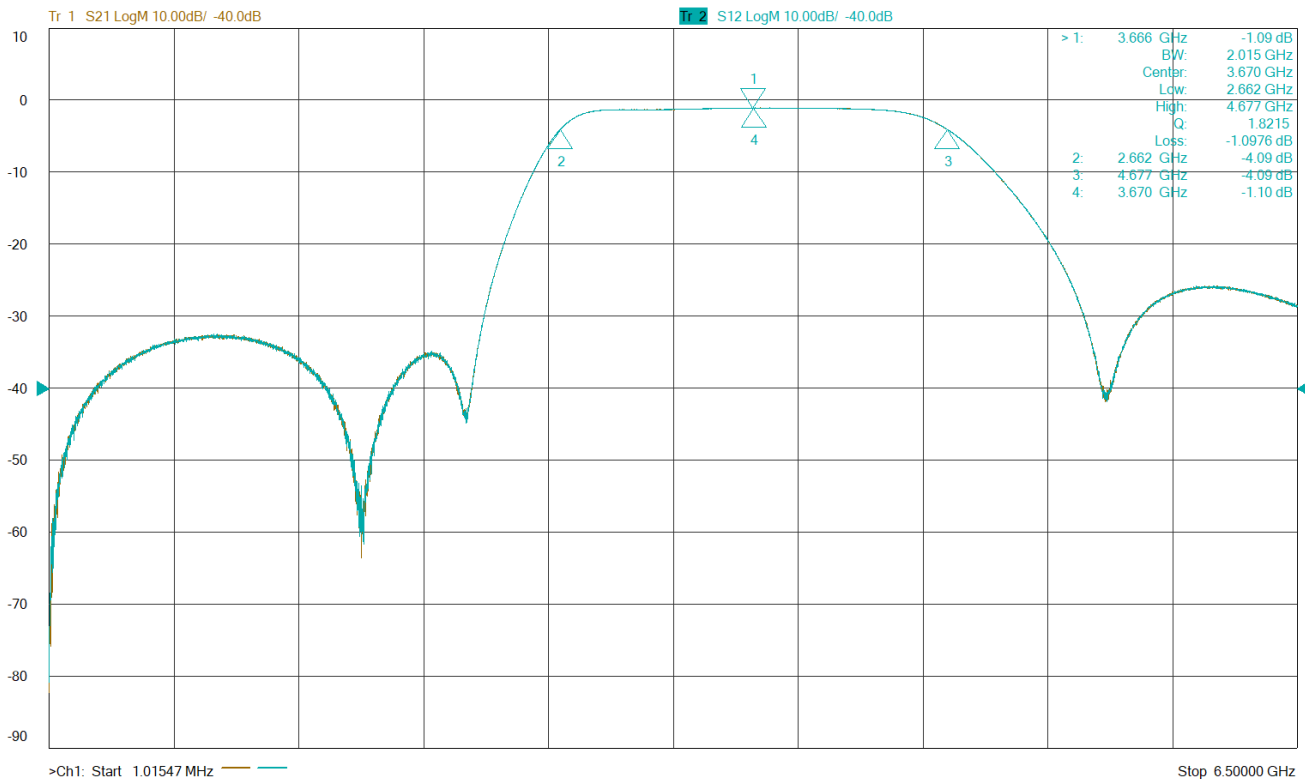
\includegraphics[width=0.9\textwidth]{img/bandpass_S12.png}
\end{figure}
\begin{equation*}
BW=\SI{2.015}{\GHz},\quad f=\SIrange{2.66}{4.67}{\GHz}
\end{equation*}
\begin{center}
$S_{21} \approx S_{12} \Rightarrow$ Reciprocal
\end{center}
\end{frame}

\begin{frame}[t,fragile]{Band Pass Filter (2) - Input/Output Reflection $S_{11}$, $S_{22}$}
\begin{figure}
  \centering
  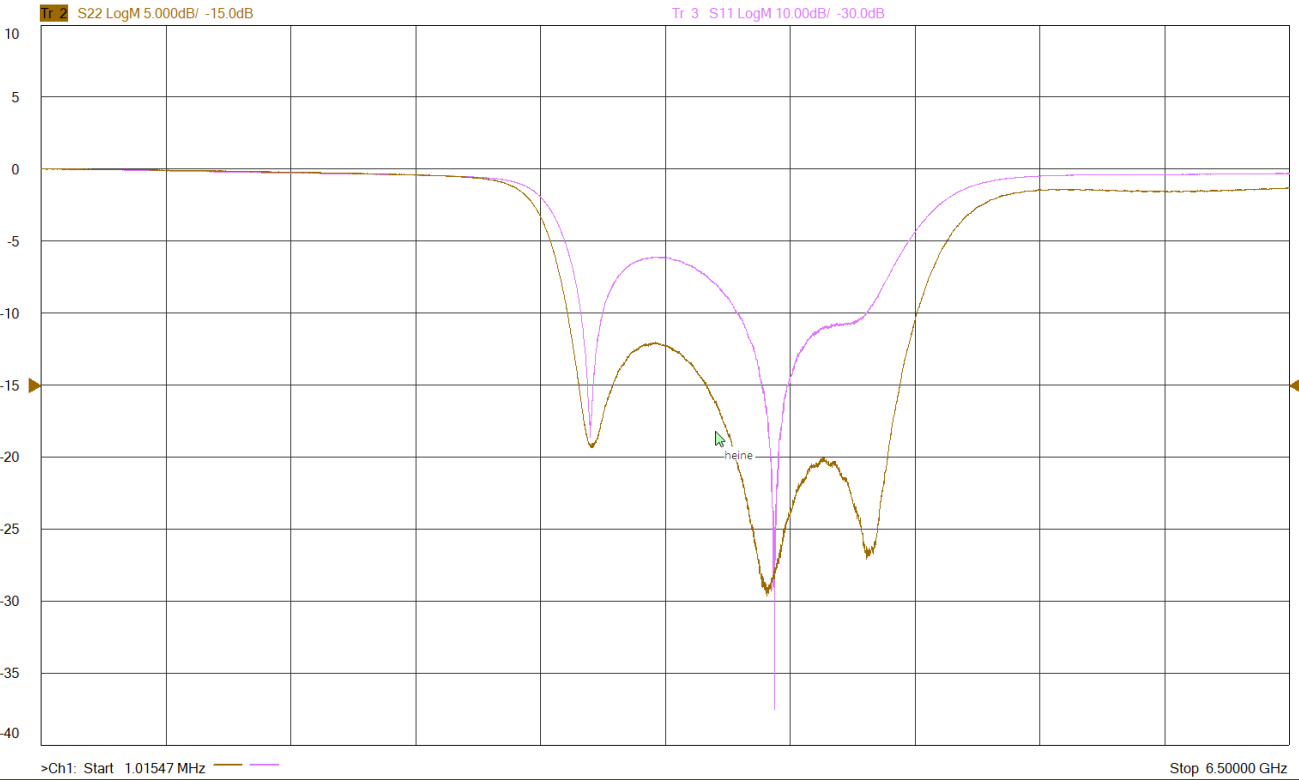
\includegraphics[width=0.9\textwidth]{img/bandpass_S11S22.png}
\end{figure}
\begin{center}
$S_{11} \neq S_{22} \Rightarrow$ Non symmetric
\end{center}
\end{frame}

\begin{frame}[t,fragile]{Band Pass Filter (3) - Phase $\angle S_{12}$}
\begin{figure}
  \centering
  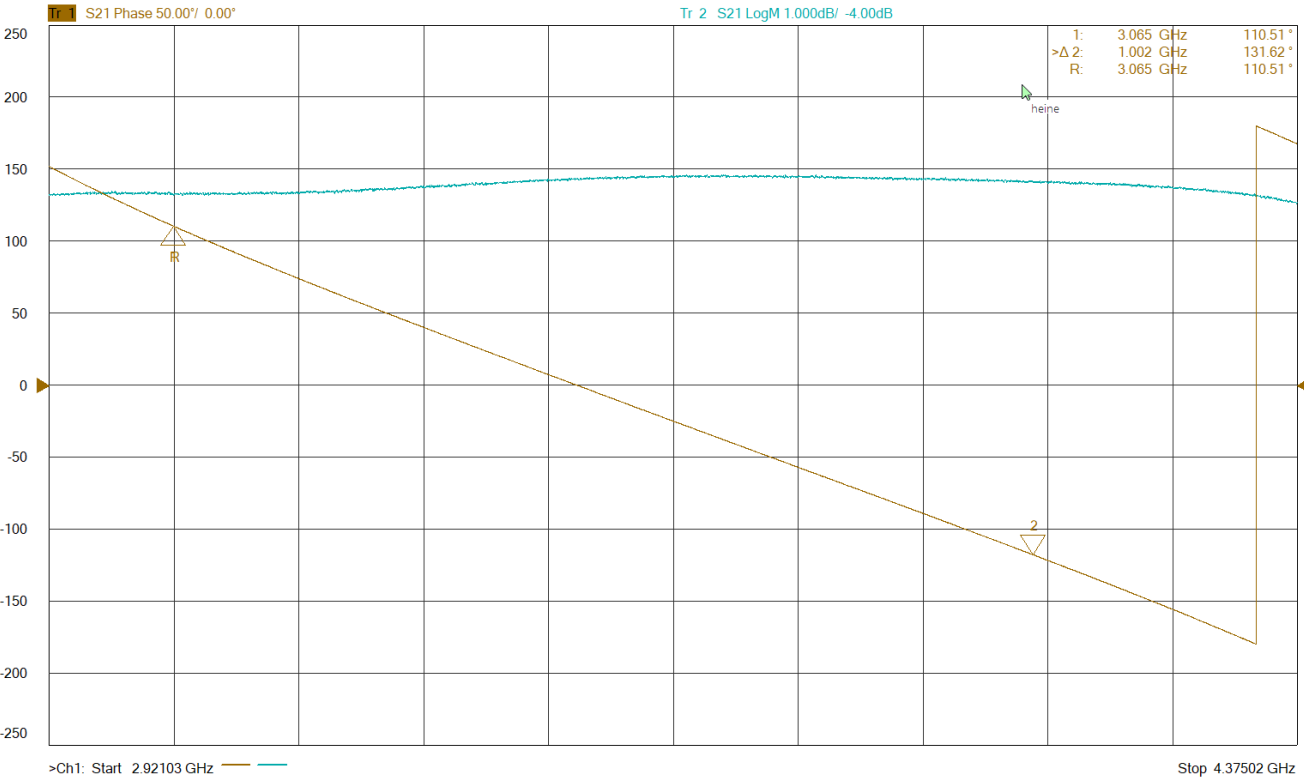
\includegraphics[width=0.9\textwidth]{img/bandpass_phase.png}
\end{figure}
\begin{equation*}
t_g = - \frac{\text{d}}{\text{d}\omega} \angle S_{12} \approx -\frac{\Delta \angle S_{12} \;[\si{\radian}]}{\Delta \omega} = \frac{(\SI{360}{\degree}-\SI{131.62}{\degree})\cdot \nicefrac{\pi}{180}}{2\pi\cdot\SI{1.002}{\GHz}} = \SI{633}{\pico\second}
\end{equation*}
\end{frame}

\begin{frame}[t,fragile]{Band Pass Filter (4) - Group Delay $t_g$}
\begin{figure}
  \centering
  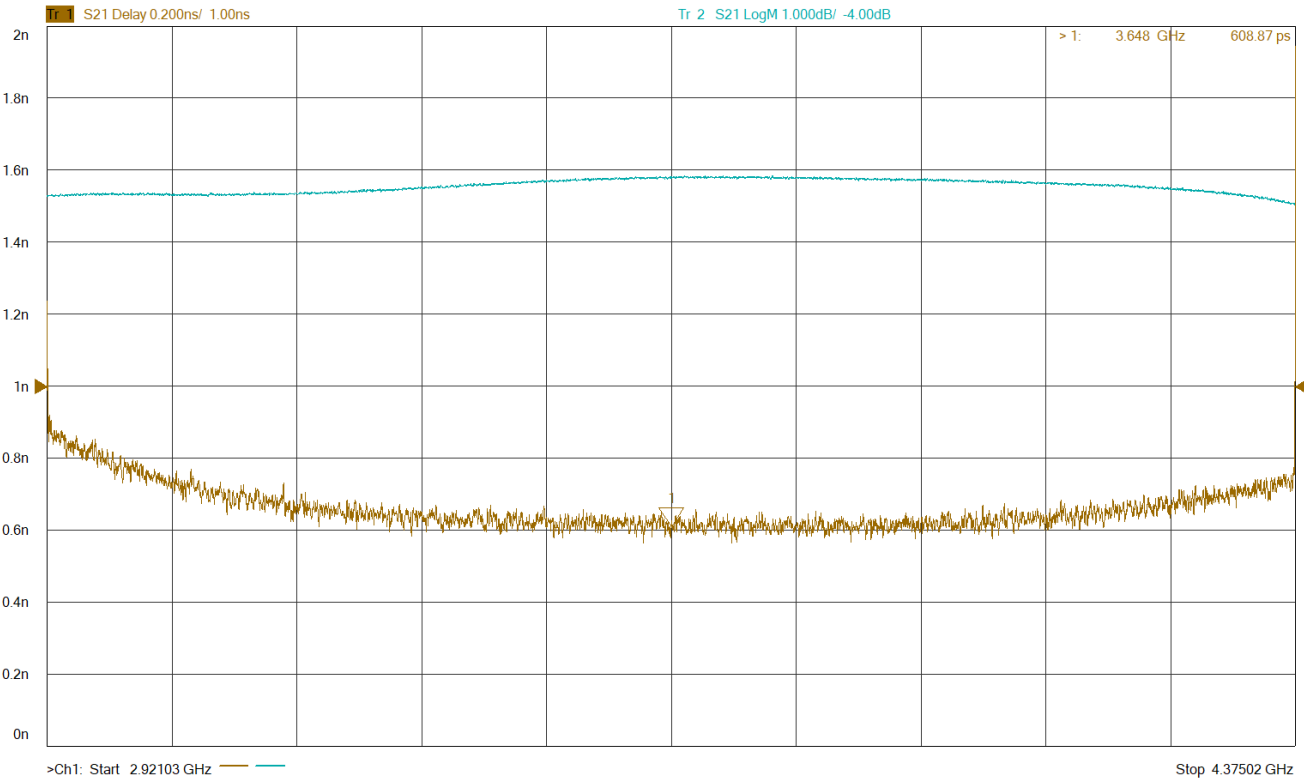
\includegraphics[width=0.9\textwidth]{img/bandpass_groupdelay.png}
\end{figure}
\begin{equation*}
\text{From group delay plot: }t_g = \SI{608.87}{\pico\second}
\end{equation*}
\end{frame}


\subsection{Strip-Line BPM}
\begin{frame}[t,fragile]{Strip-Line BPM (1) - Intro}

Reflectometry for 500 MHz and 50 Ohm
\begin{itemize}
\item[a] Connector
\item[b] Strip line
\begin{itemize}
\item Four 14cm strips
\item Short-circuit termination
\end{itemize}
\end{itemize}

\begin{figure}
  \centering
  \subfloat[Strip line: image and circuit]{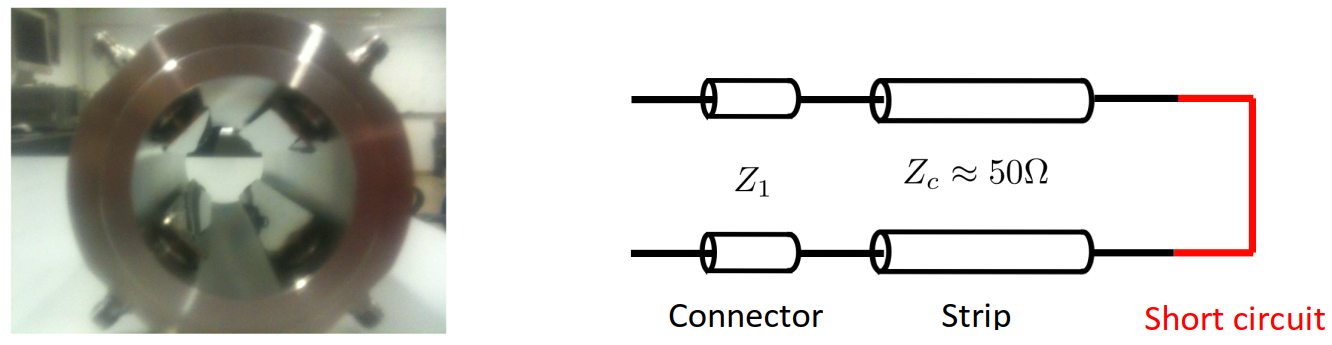
\includegraphics[width=0.9\textwidth]{2_1}}\quad
%  \subfloat[b]{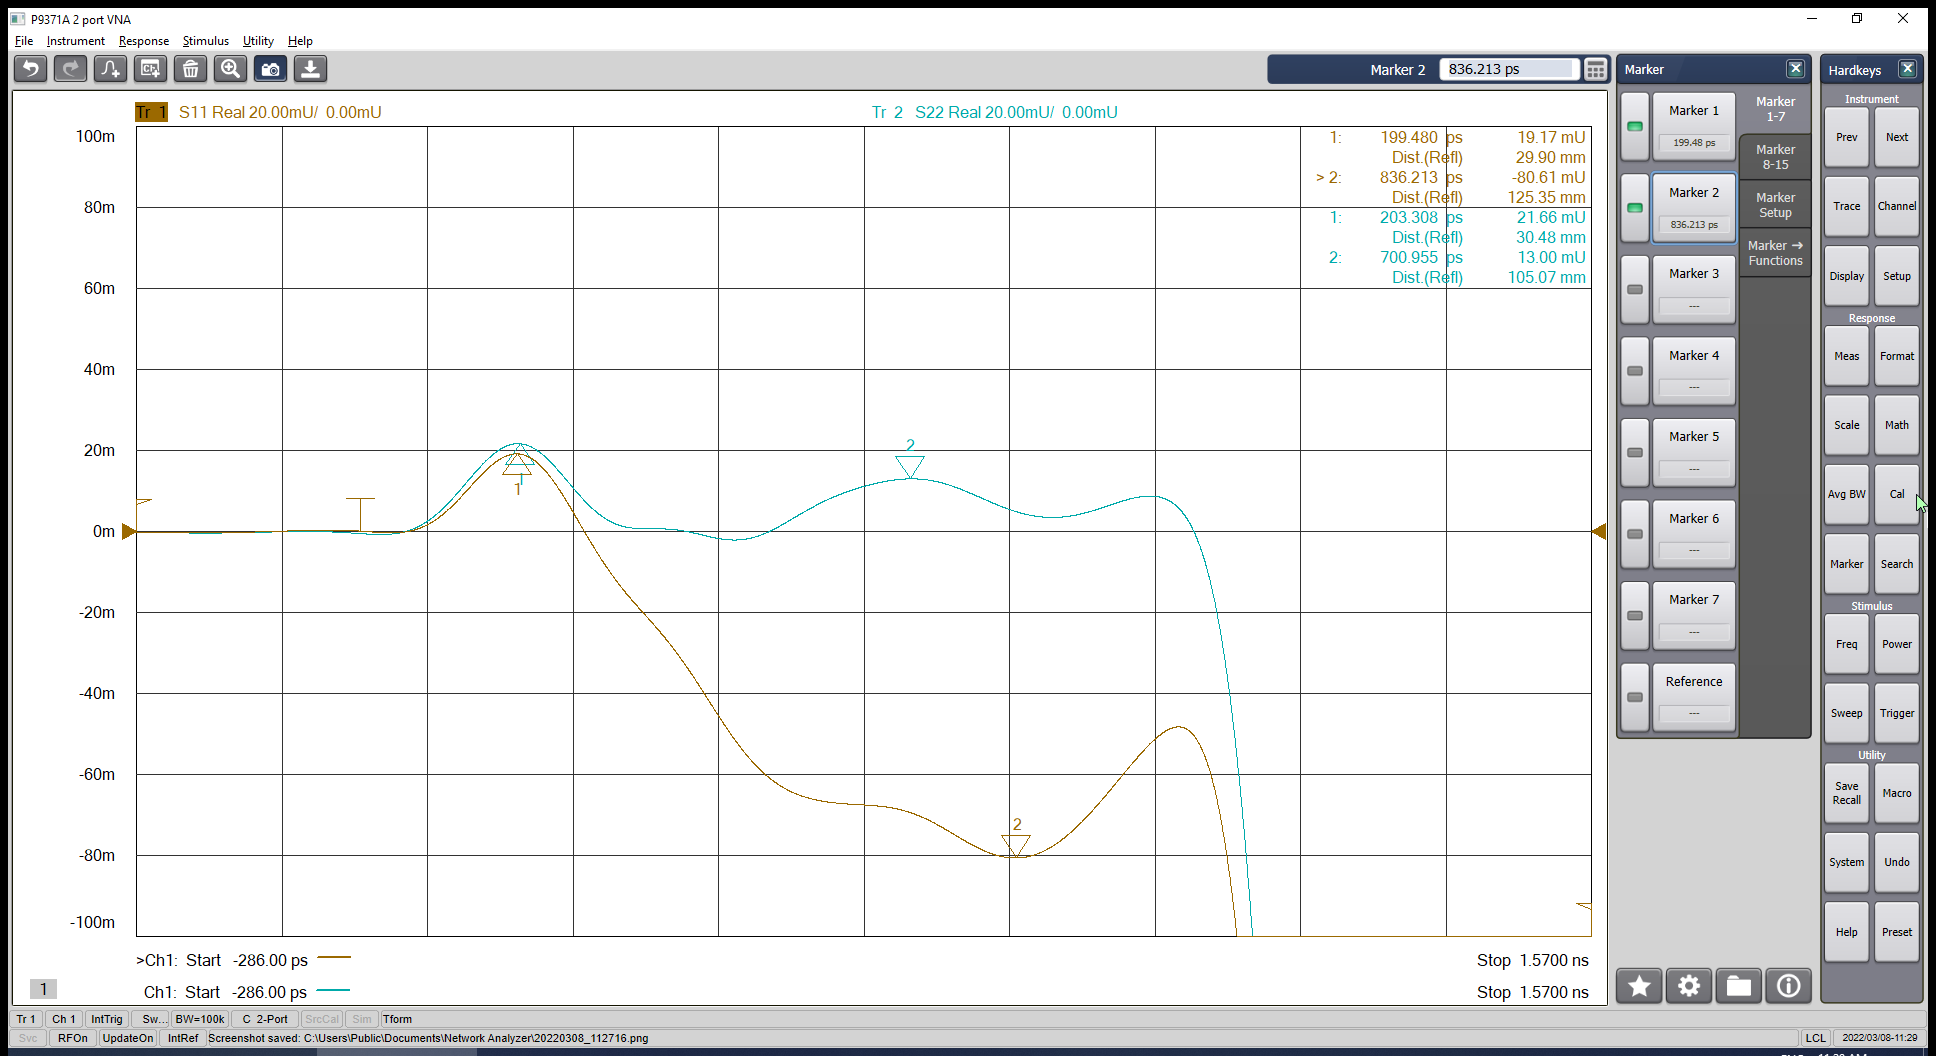
\includegraphics[width=0.45\textwidth]{2_S11_TD}}\\
%  \subfloat[Caption c]{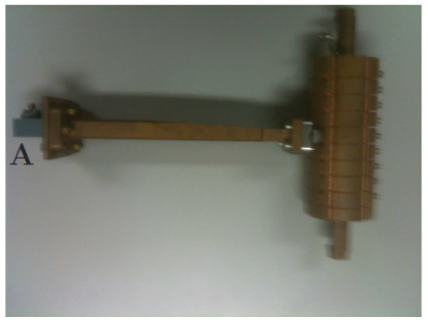
\includegraphics[width=0.28\textwidth]{3_1}}\quad
%  \subfloat[Caption d]{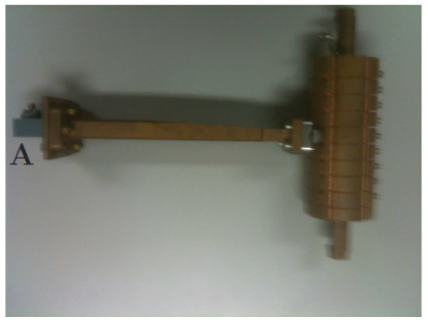
\includegraphics[width=0.28\textwidth]{3_1}}
\end{figure}

\end{frame}

\begin{frame}[t,fragile]{Strip-Line BPM (2) - Time Domain Reflectometry}
\begin{itemize}
\item Measuring S11 in time domain to check acceptance criteria
\begin{itemize}
\item[a] Connector: $+ 50 mU$ 
\item[b] Strip line: $-/+ 20mU$
\end{itemize}
\item Strip line \textit{blue} in specs, \textit{gold} not
\end{itemize}

\begin{figure}
  \centering
  \subfloat[TDR Aim]{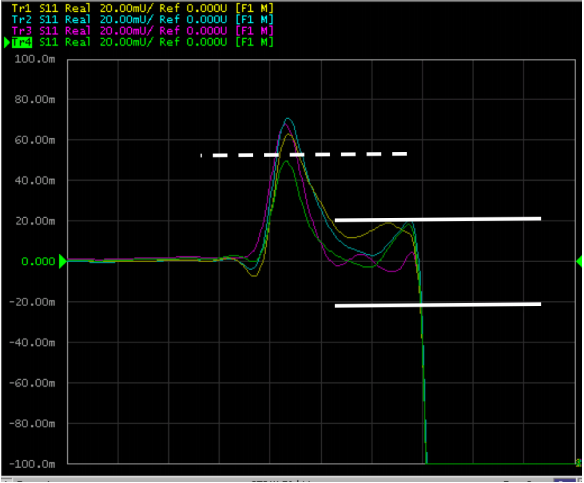
\includegraphics[width=0.4\textwidth]{2_2}}\quad
  \subfloat[TDR Reproduced]{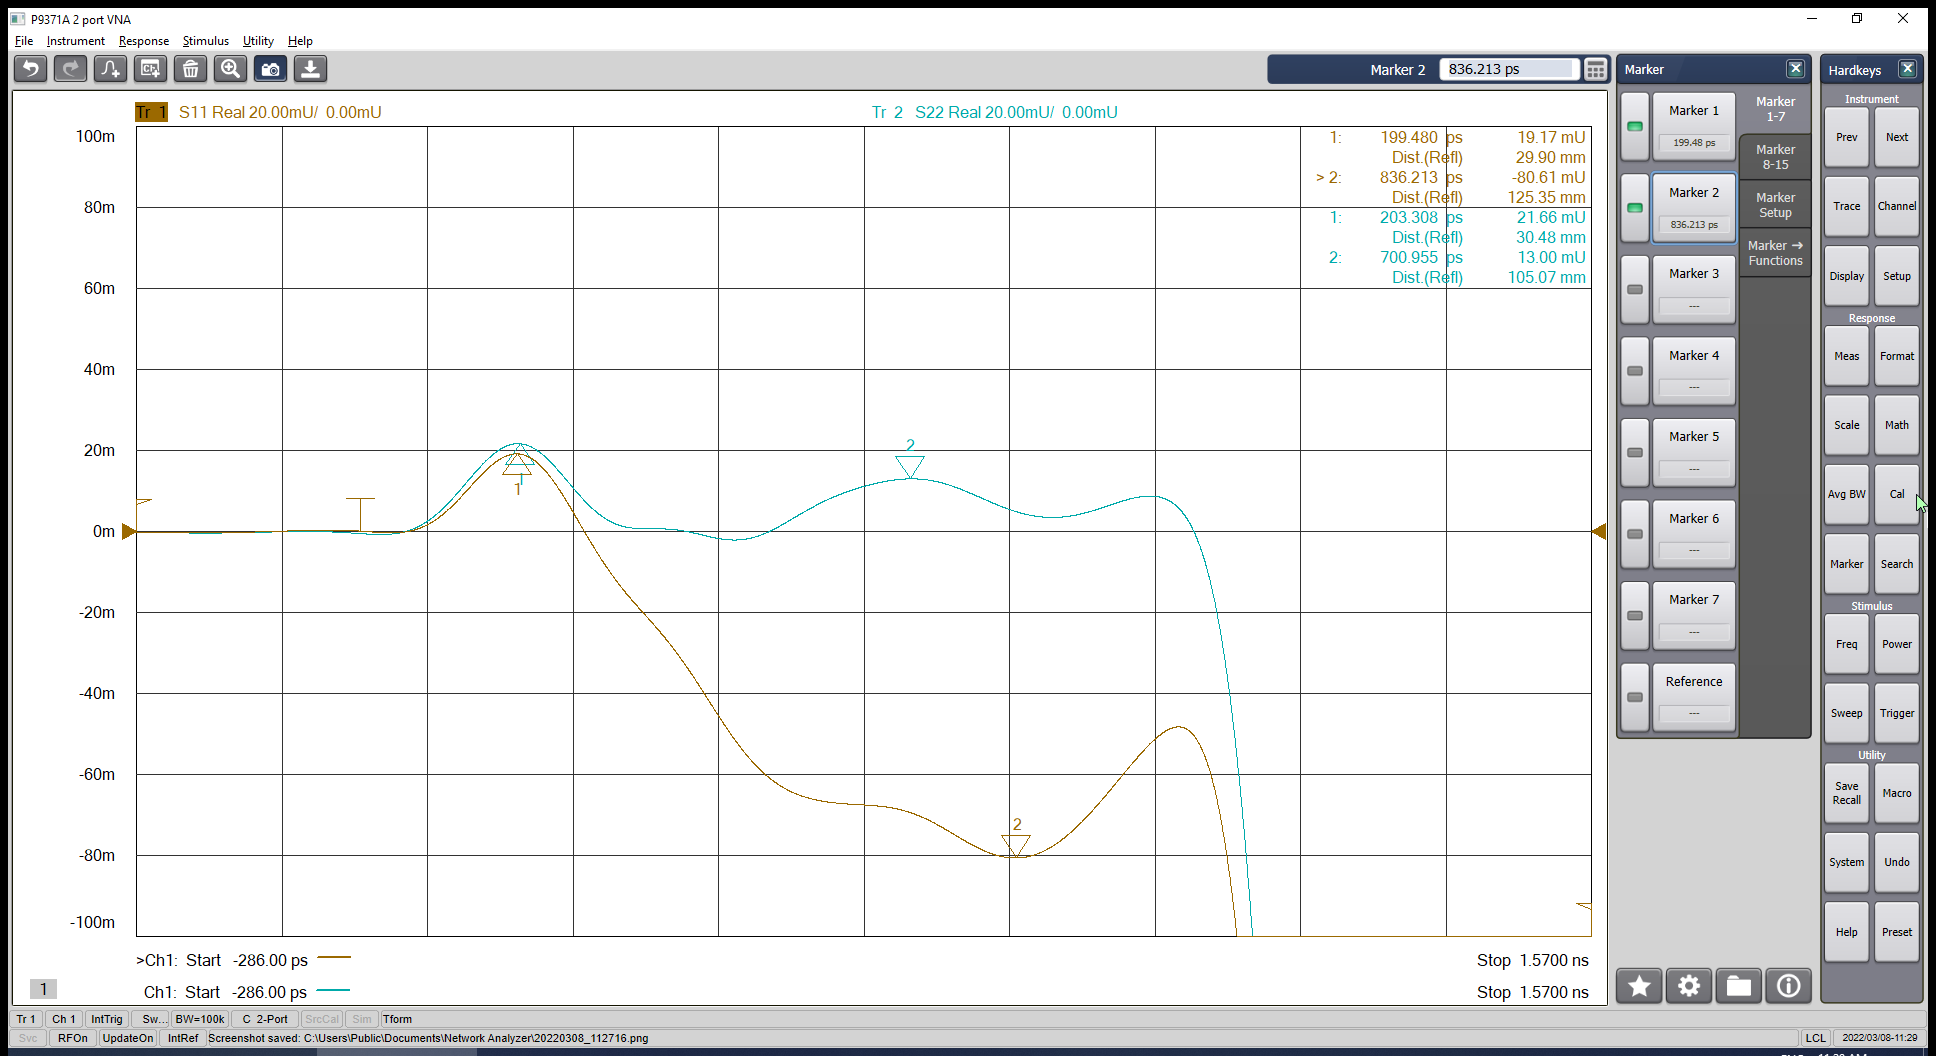
\includegraphics[width=0.55\textwidth]{2_S11_TD}}\\
%  \subfloat[Caption c]{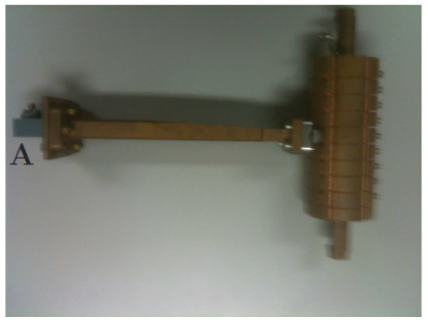
\includegraphics[width=0.28\textwidth]{3_1}}\quad
%  \subfloat[Caption d]{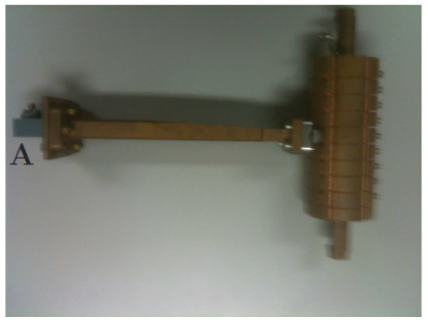
\includegraphics[width=0.28\textwidth]{3_1}}
\end{figure}

\end{frame}

\begin{frame}[t,fragile]{Strip-Line BPM (3) - Frequency Domain Characterization}
\begin{itemize}
\item Strip-line length from S11
\begin{itemize}
\item from S11: $1.086 ns$, $162.77 mm$

\item from phase: $1.218 ns$, $182.58 mm$
\item from group delay: $1.32  ns$, $197.87 mm$
\end{itemize}
\item Cross-talk from S21
\begin{itemize}
\item Maximum reflection of $ -25.25 dB$ at $797.68 MHz$ 
\item Reflection of $ -53.06 dB$ at operation frequency $ 500.00 MHz$
\end{itemize}
\end{itemize}

\begin{figure}
  \centering
  \subfloat[Calculation from S11]{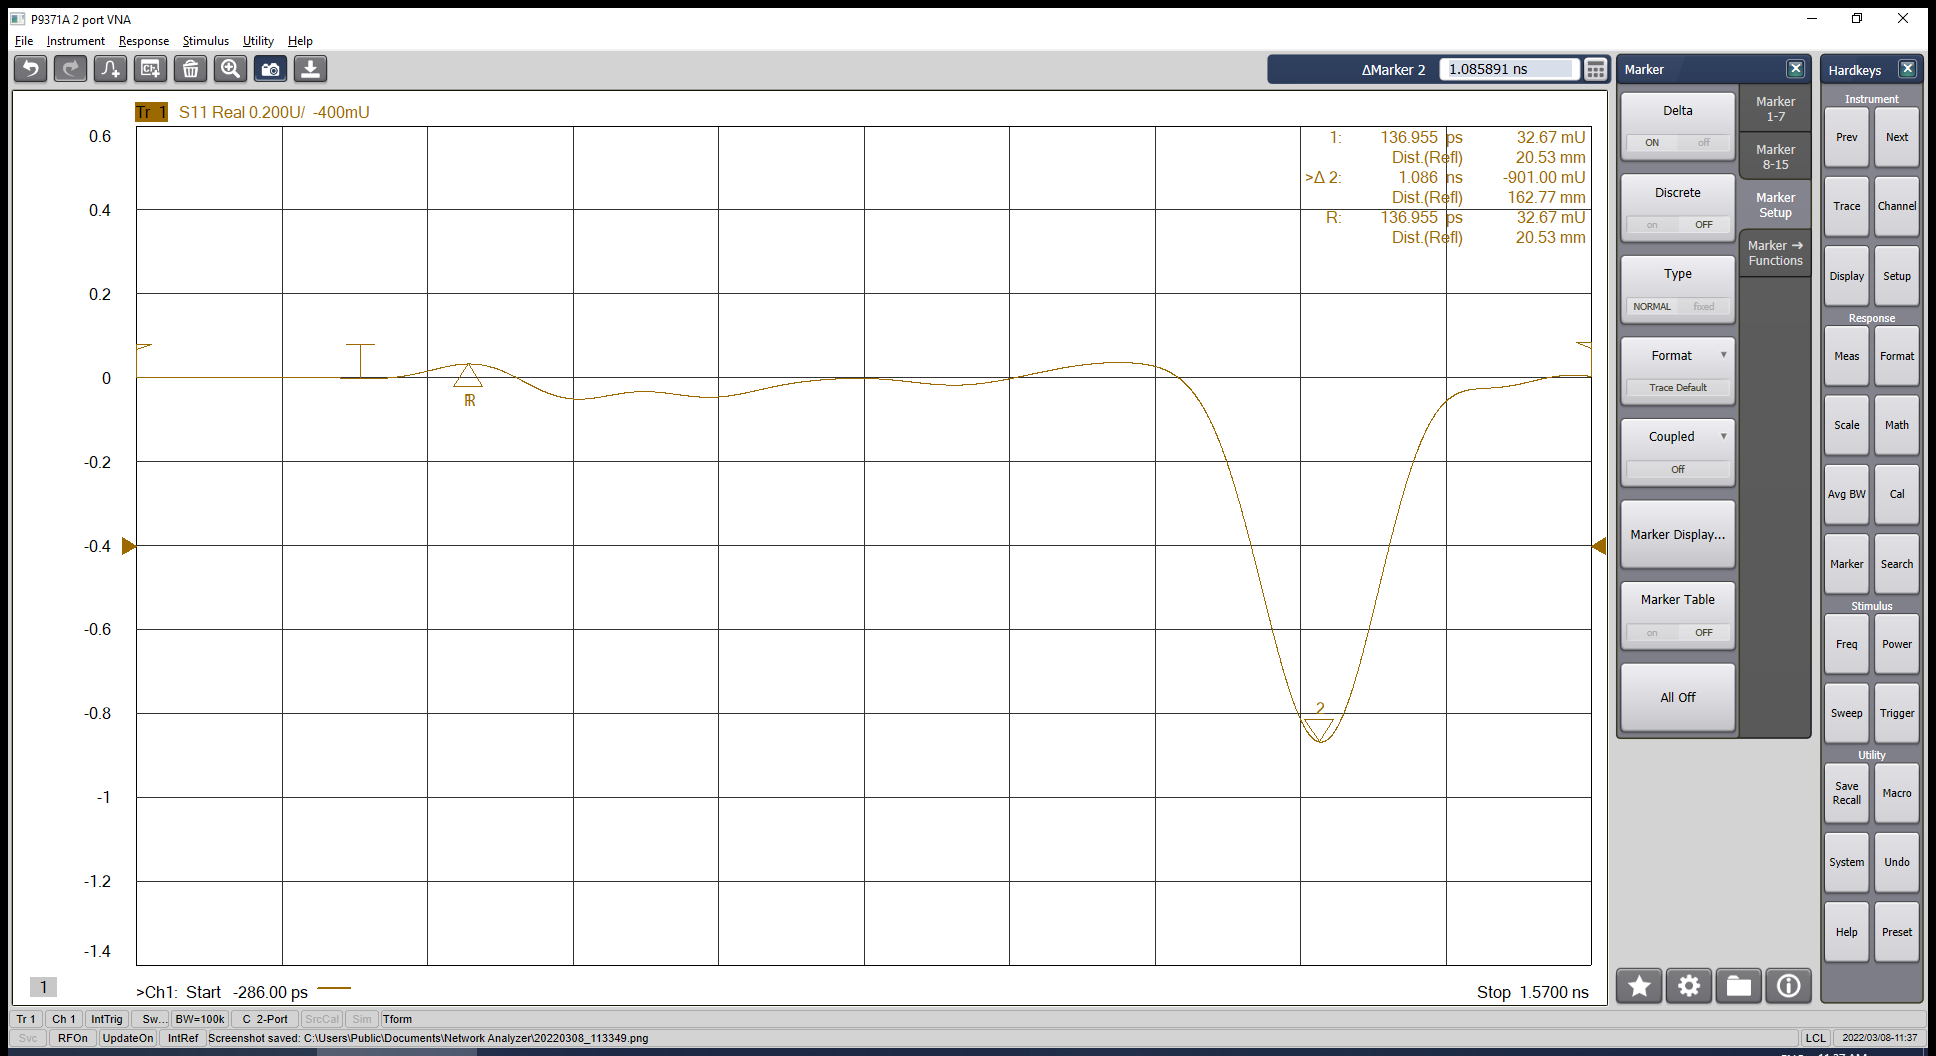
\includegraphics[width=0.48\textwidth]{2_length}}\quad
  \subfloat[Calculation from phase]{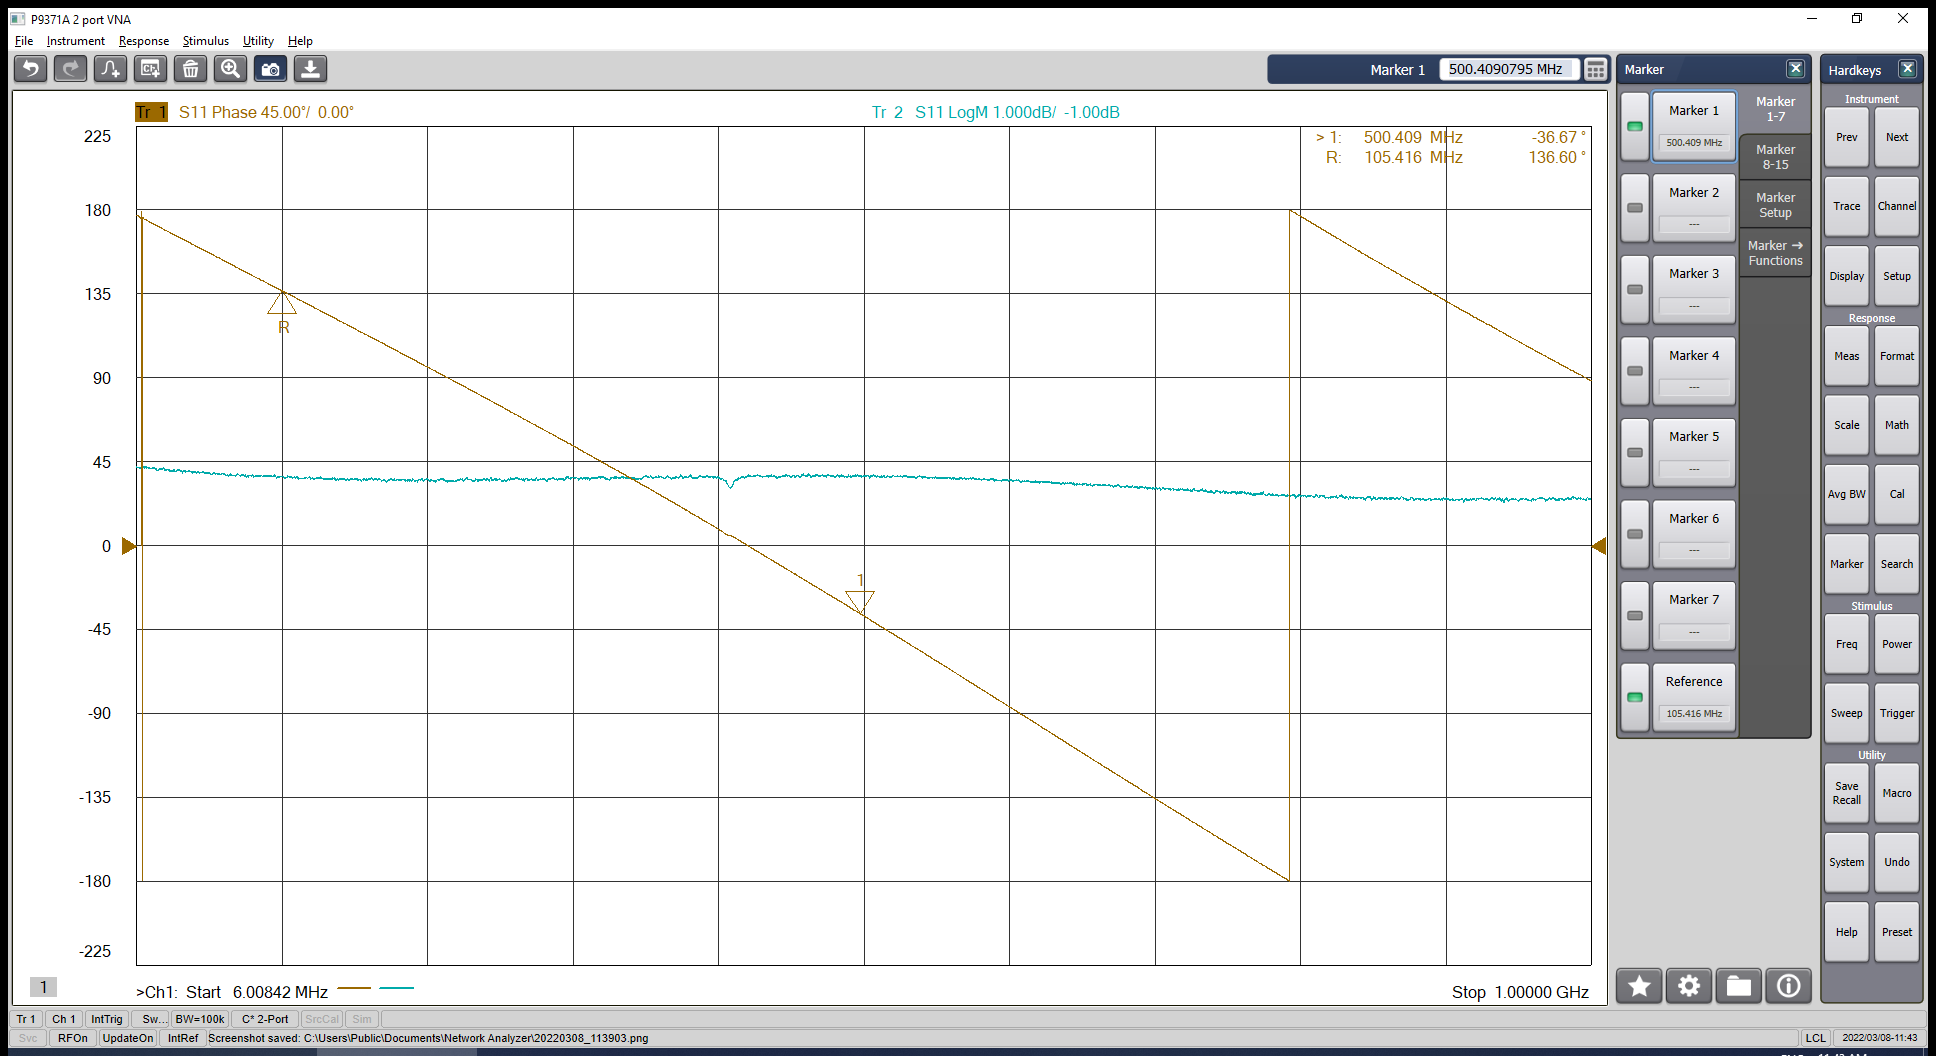
\includegraphics[width=0.48\textwidth]{2_phase}}\\
\end{figure}

\end{frame}

%\begin{frame}[t,fragile]{Strip-Line BPM (4) - Strip Line Length}
%\begin{itemize}
%\item Strip-line length from S11
%\begin{itemize}
%\item $1.086 ns$ translates to $162.77 mm$
%\end{itemize}
%\item Comparision with group delay: $1.218 ns$, $182.58 mm$
%\item Cross-talk from S21
%\begin{itemize}
%\item Maximum reflection of $ -25.25 dB$ at $797.68 MHz$ 
%\item Reflection of $ -53.06 dB$ at operation frequency $ 500.00 MHz$
%\end{itemize}
%\end{itemize}
%
%\begin{figure}
%  \centering
%  \subfloat[TDR Aim]{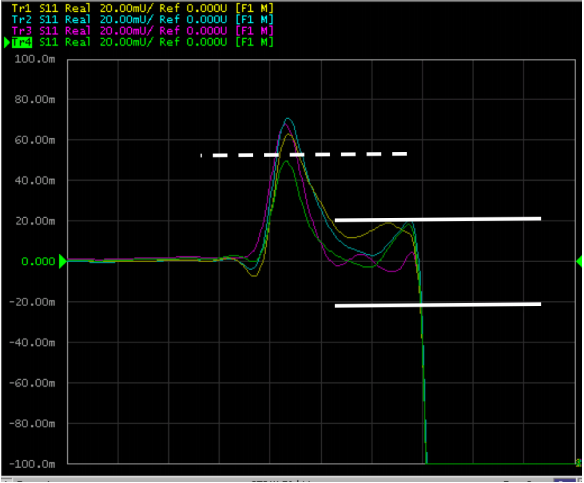
\includegraphics[width=0.4\textwidth]{2_2}}\quad
%  \subfloat[TDR Reproduced]{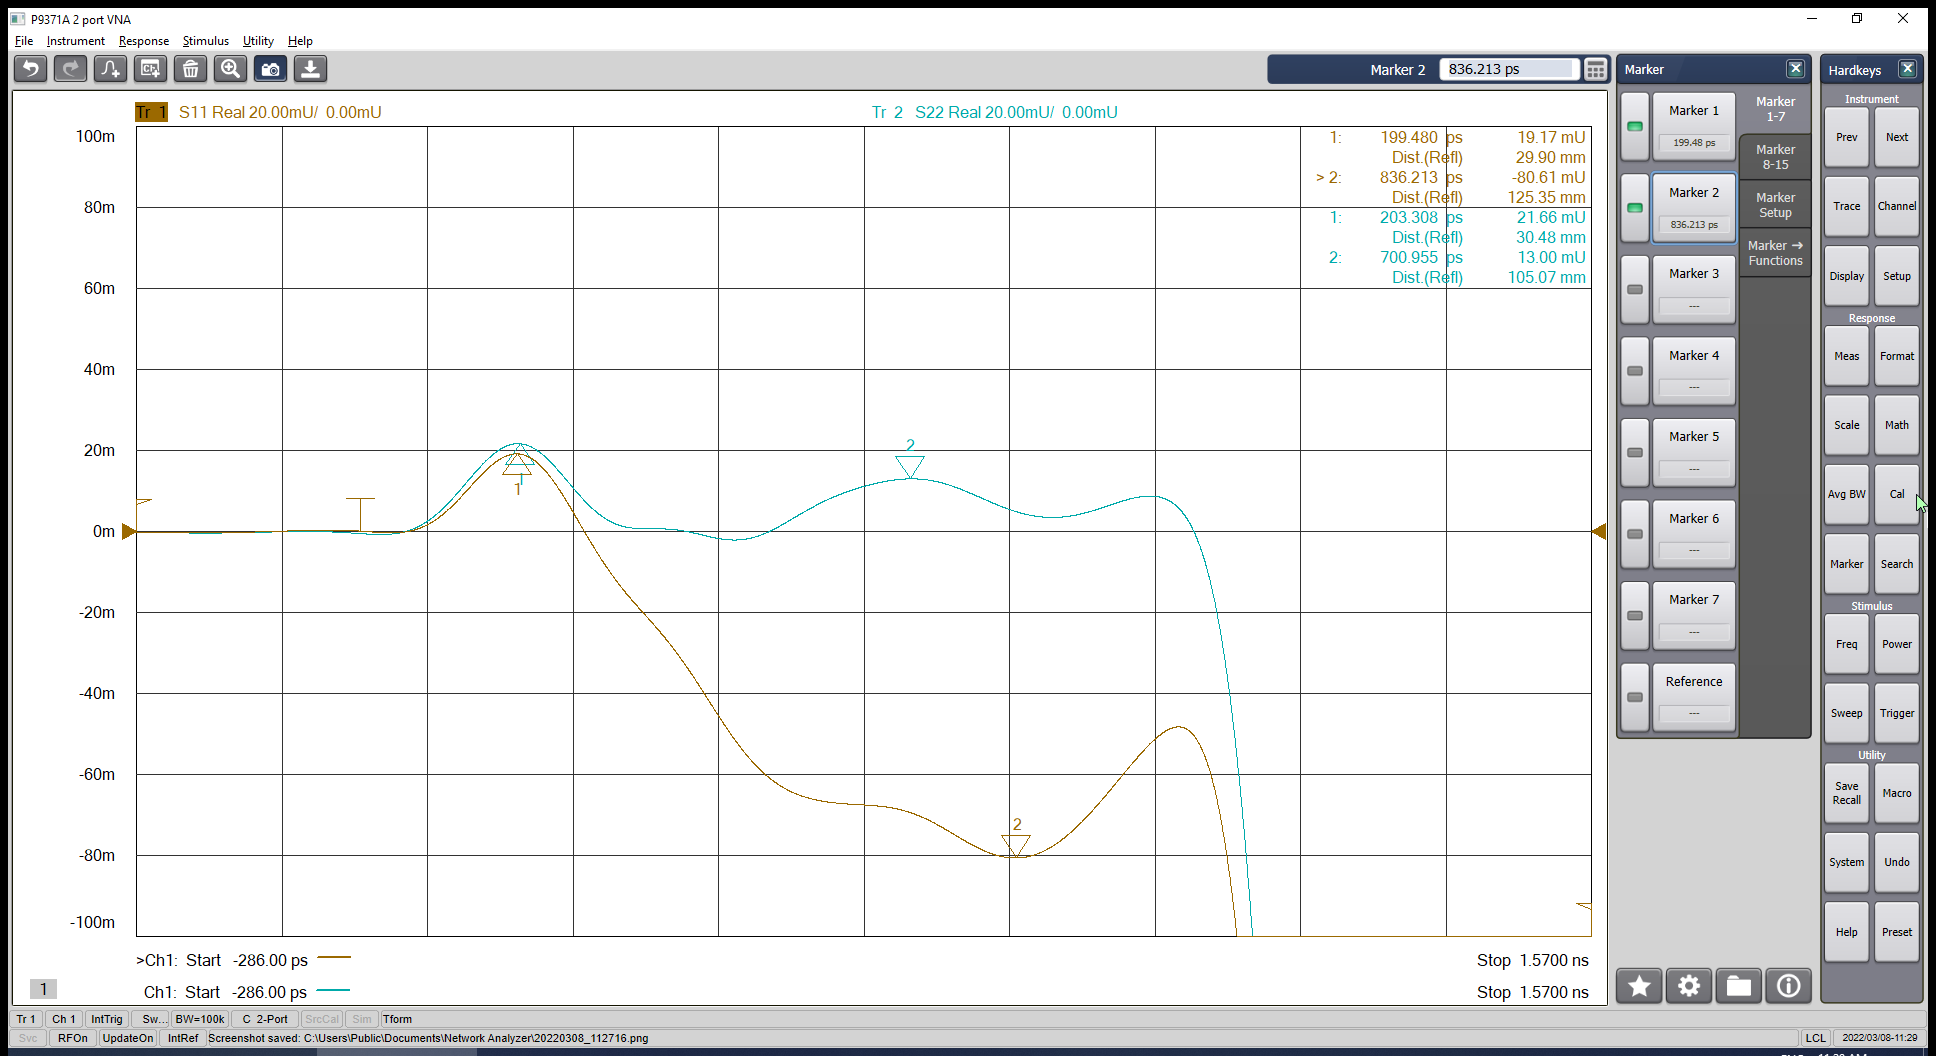
\includegraphics[width=0.55\textwidth]{2_S11_TD}}\\
%\end{figure}
%
%\end{frame}

\subsection{RF - Cavaties}
\begin{frame}[t,fragile]{RF - cavaties (1) - Intro}
\begin{itemize}
\item Multi cell cavity in X-band
\item Operating mode at 11.424 GHz
\item Under coupled antenna
\end{itemize}

\begin{figure}
  \centering
  \subfloat[Multi cell cavity]{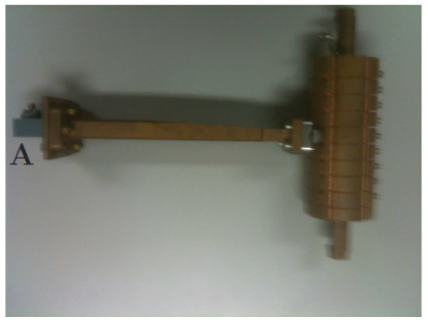
\includegraphics[width=0.48\textwidth]{3_1}}\quad
  \subfloat[Setup]{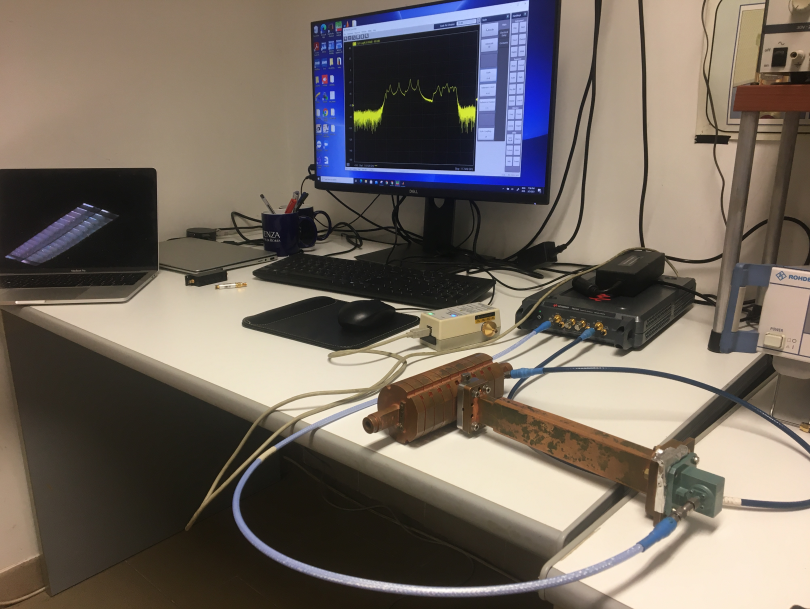
\includegraphics[width=0.48\textwidth]{3_1_2}}\\
\end{figure}

\end{frame}

\begin{frame}[t,fragile]{RF - cavaties (2) - Transmission measurement}
\begin{itemize}
\item Identify different modes 
\item Calculated Q from the $3 dB$ bandwidth: $3093$
\begin{figure}
  \centering
  \subfloat[All modes (S21)]{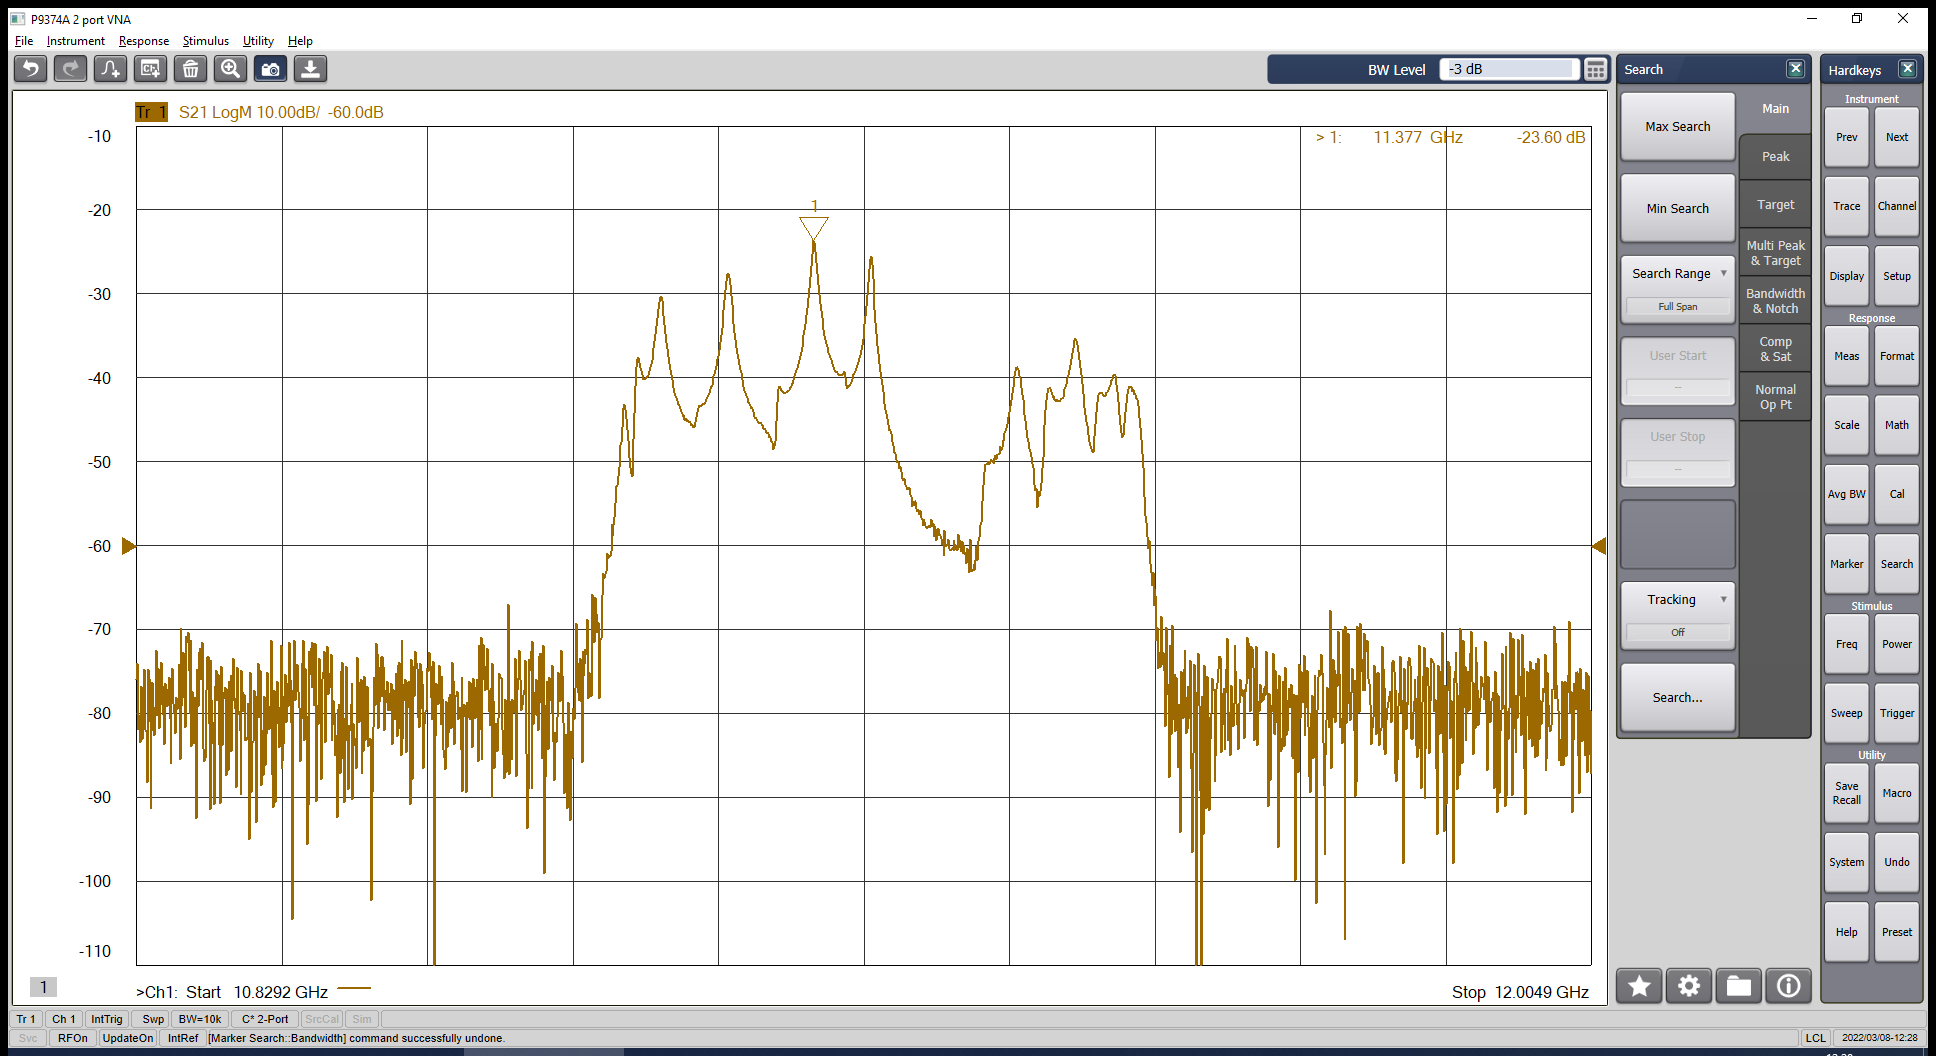
\includegraphics[width=0.45\textwidth]{3_S11_all_modes}}\quad
  \subfloat[Q for a certain mode]{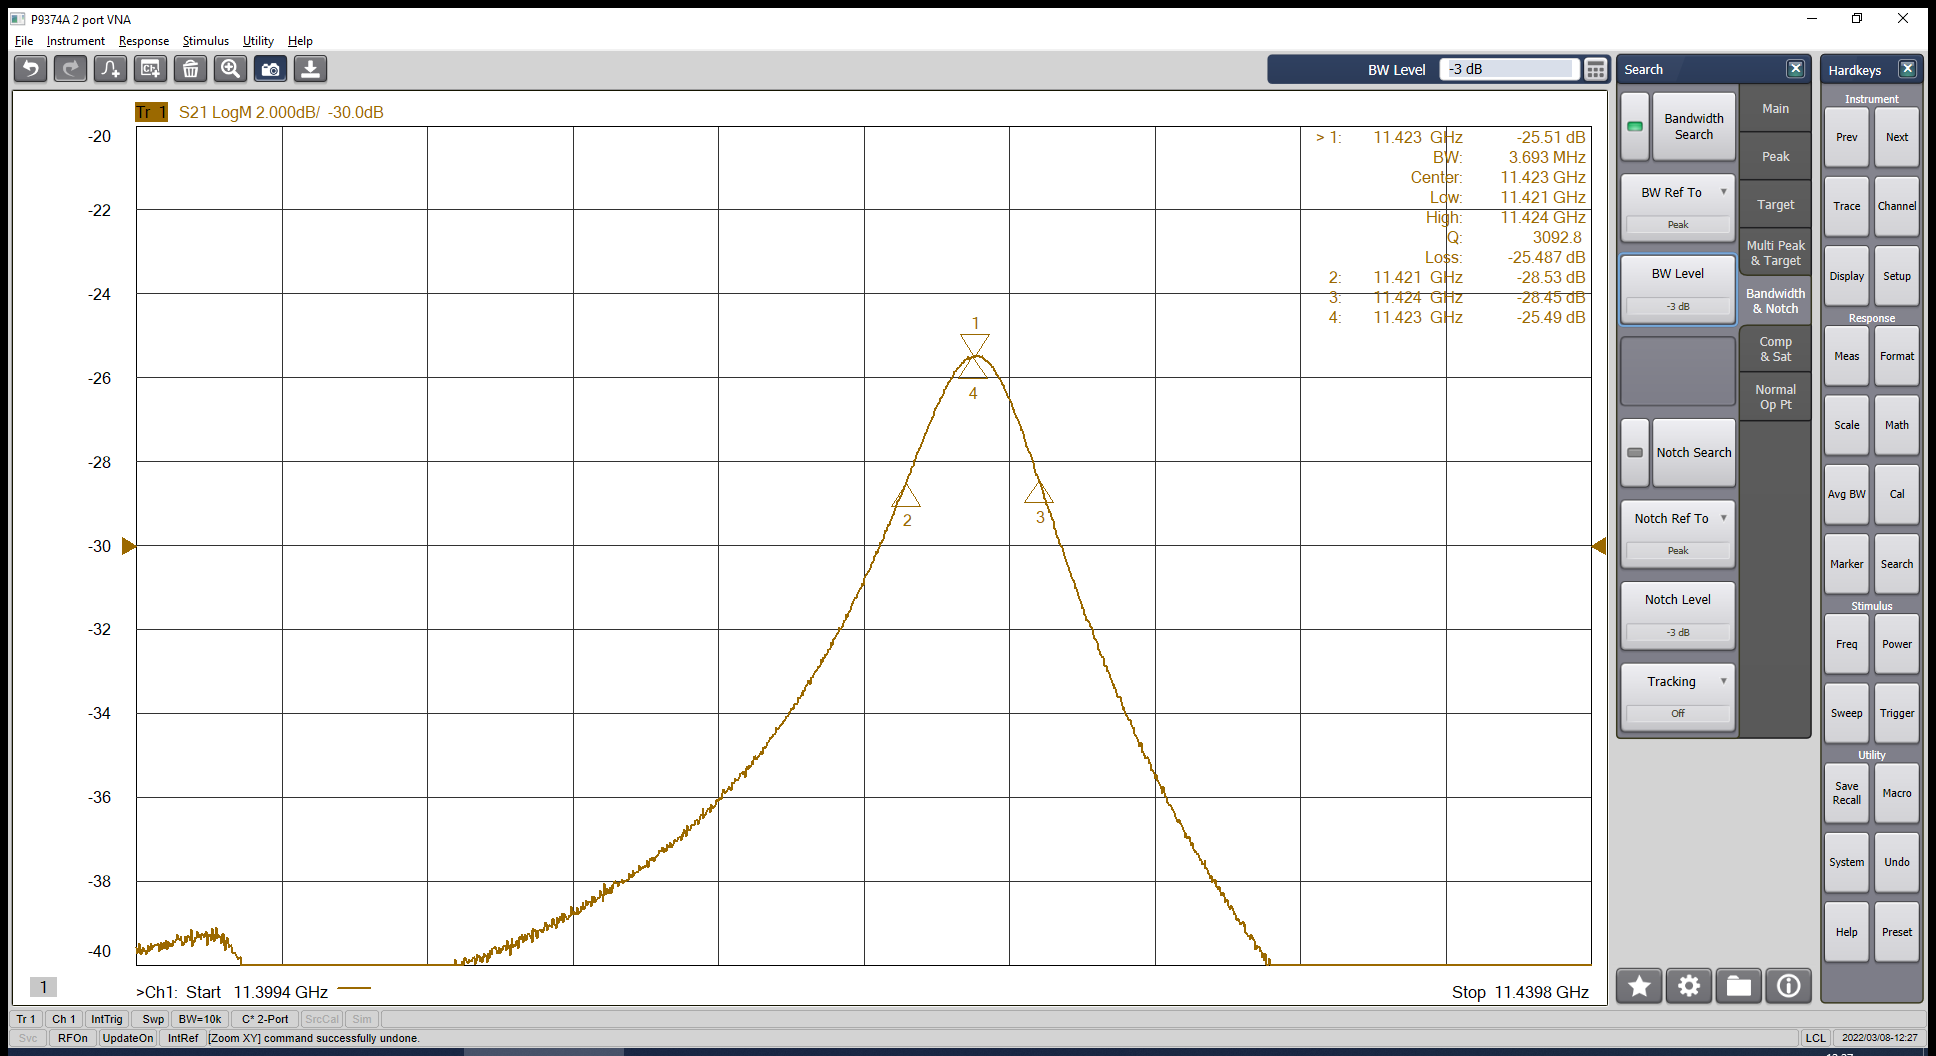
\includegraphics[width=0.45\textwidth]{3_S11_mode}}\\
\end{figure}
\end{itemize}
\end{frame}

\begin{frame}[t,fragile]{RF - cavaties (3) - Transmission measurement}
\begin{itemize}
\item Identify SWR
\item Under coupling (S11 in Smith Chart)
\begin{figure}
  \centering
  \subfloat[Caption a]{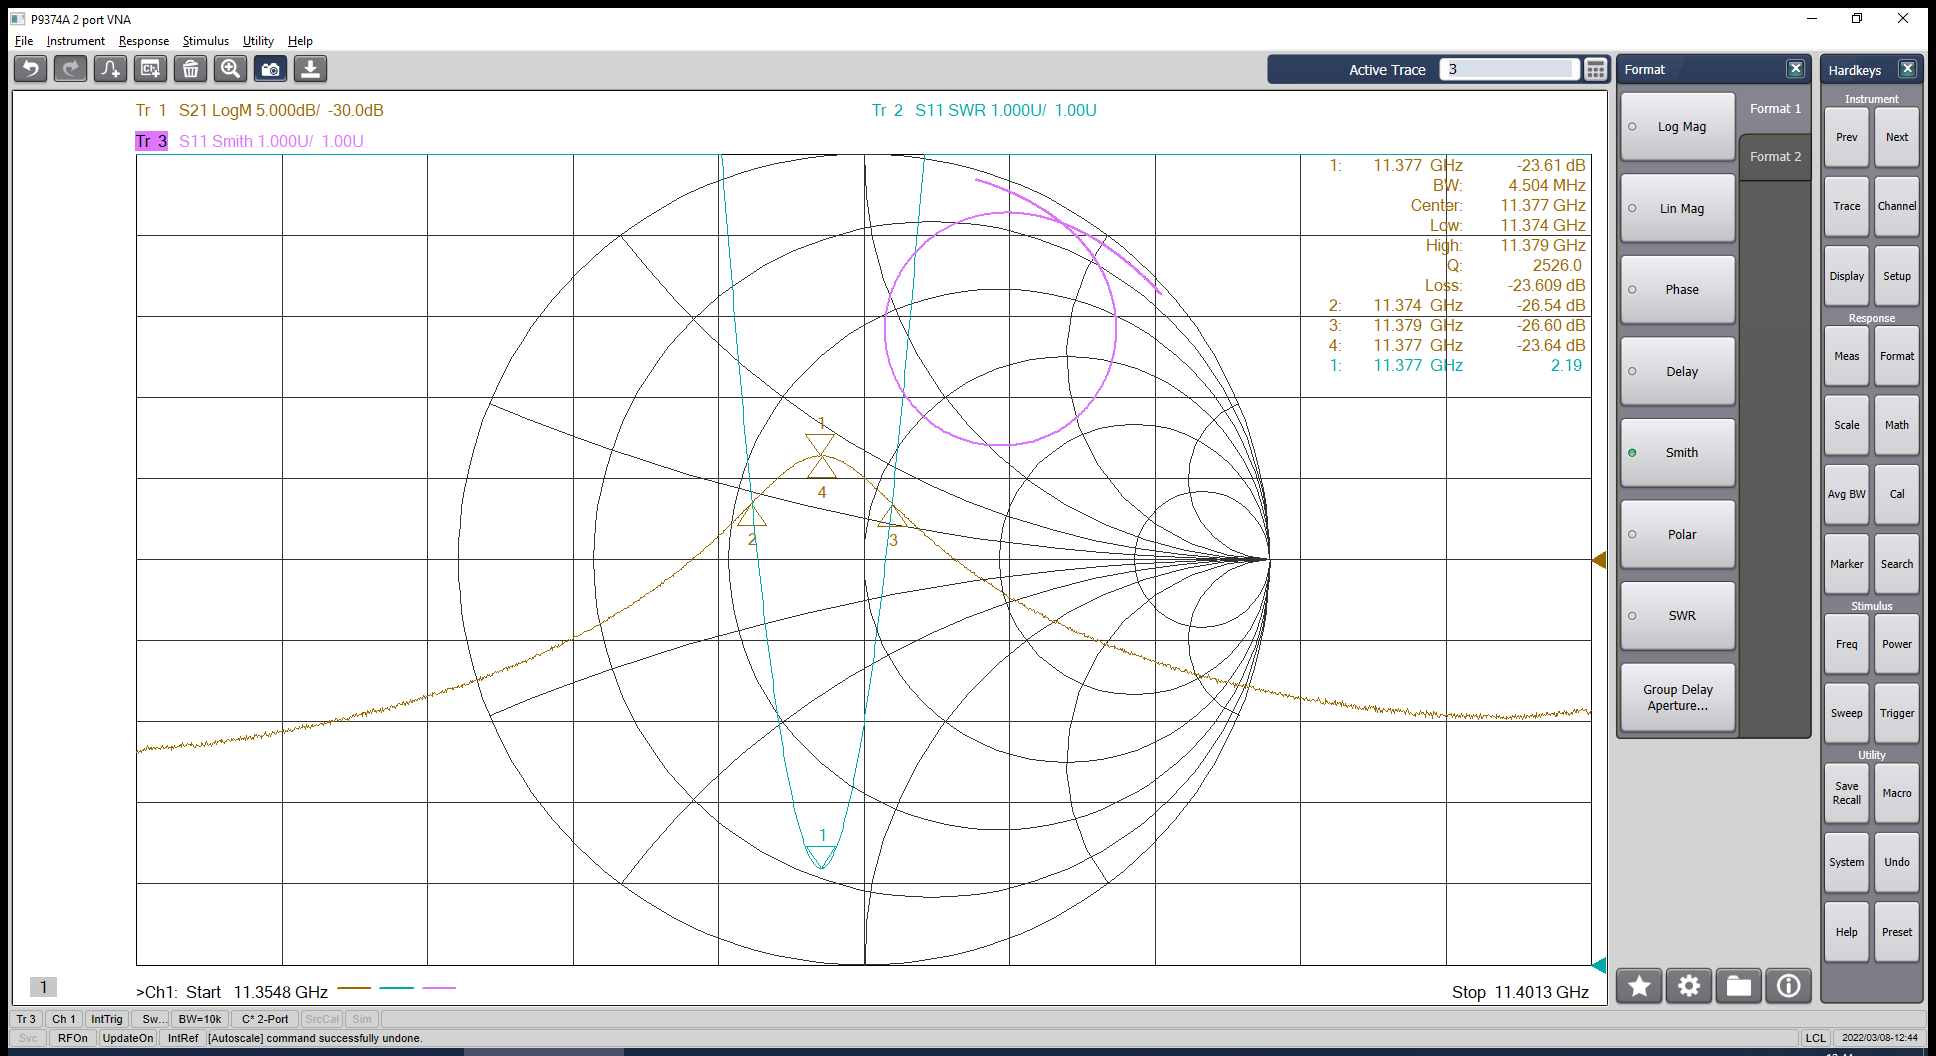
\includegraphics[width=0.45\textwidth]{3_comby_plot}}\quad
  \subfloat[Caption b]{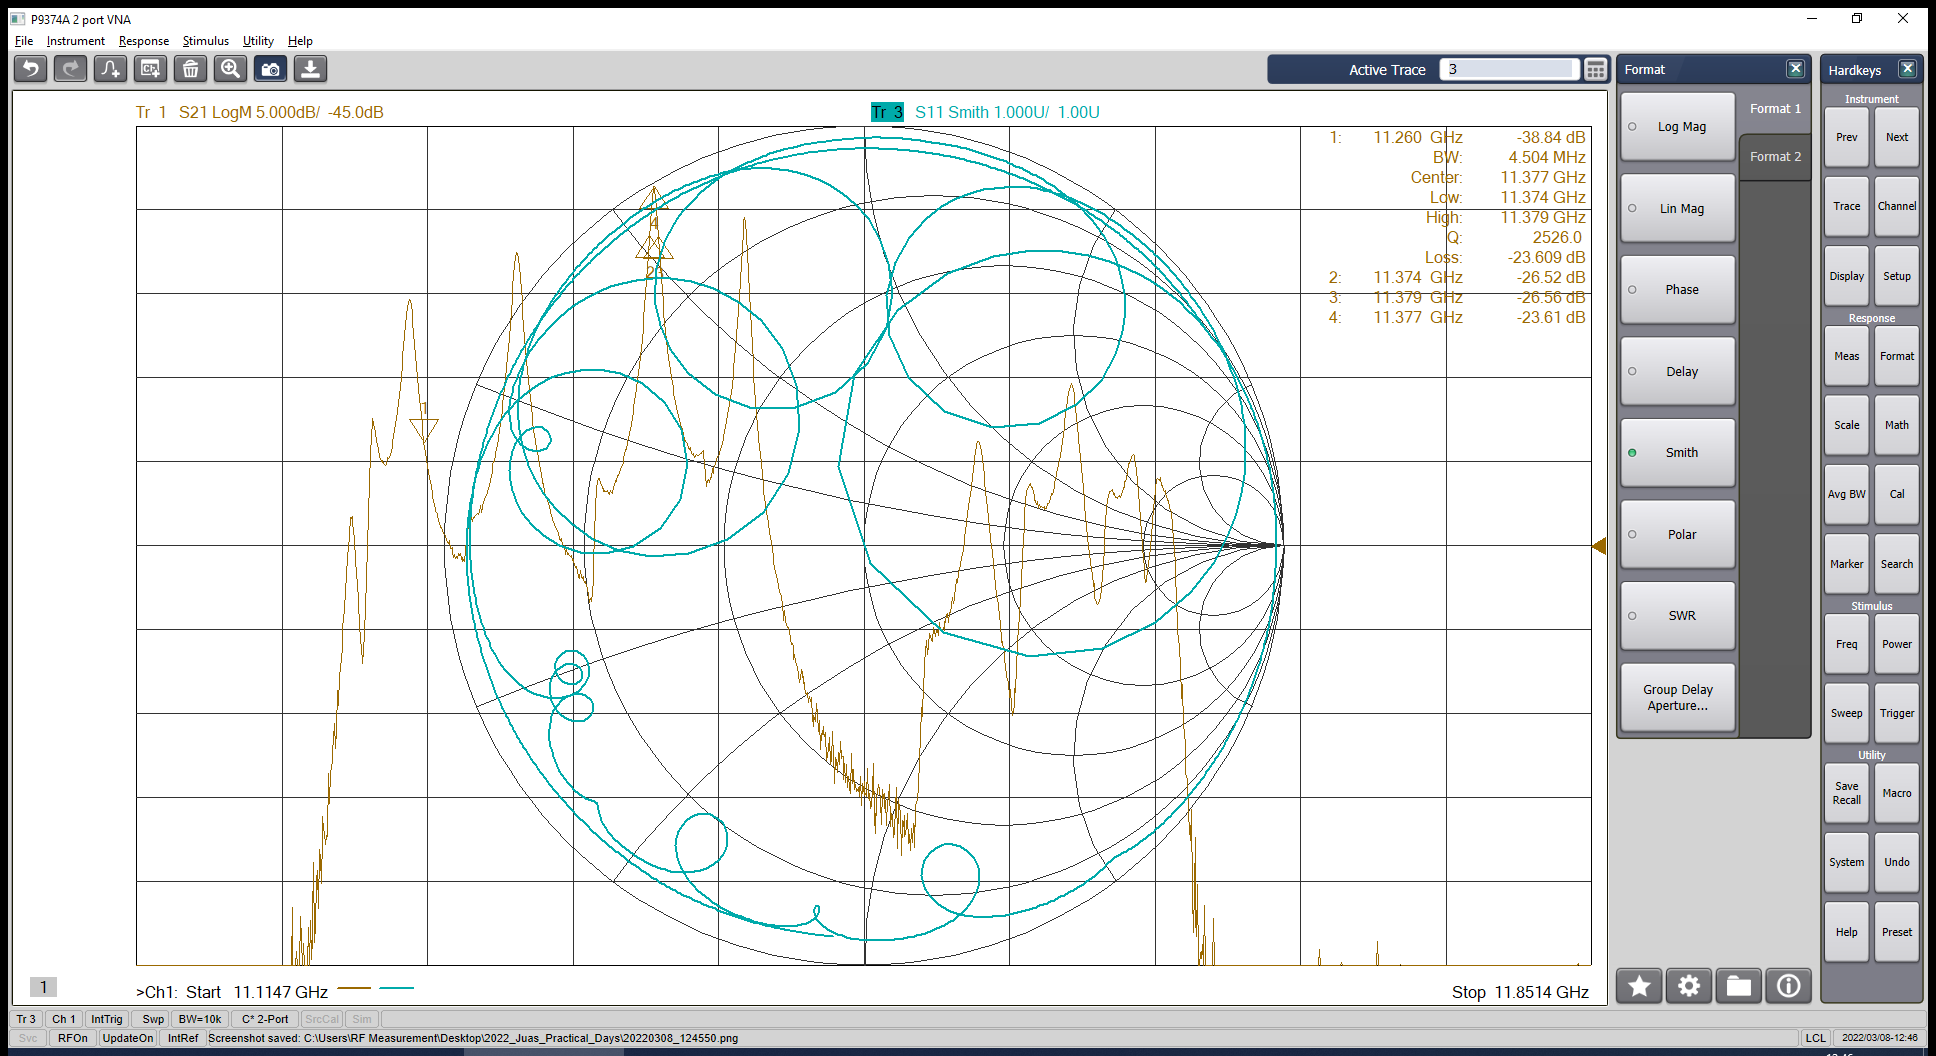
\includegraphics[width=0.45\textwidth]{3_comby_plot_all}}\\
\end{figure}
\end{itemize}
\end{frame}

\section{Afternoon Session}
\subsection{Useless Repetition}
\begin{frame}[t,fragile]{Useless Repetition (Manfred Wendt)}
\begin{itemize}
\item Stuff
\item More Stuff
\end{itemize}
\end{frame}

\subsection{Coupling of an RF Cavity}
\begin{frame}[t,fragile]{RF Cavity, Coupling, Smith Chart (Fritz Caspers)}
\begin{itemize}
\item  Two Antennas in cavaty
\begin{itemize}
\item Longitudinal field antenna
\item Coupling loop
\end{itemize}
\item Under-, over- and critical coupling
\end{itemize}
\end{frame}

\section{Resume}
\begin{frame}[t,fragile]{Resume}
\begin{itemize}
\item Network Analyser
\begin{itemize}
\item Time and Frequency Domain
\item Scattering parameter, Impedance, SWR, phase
\item Calculation of Q, reflexion coefficient
\end{itemize}
\item Spectrum Analyser (Modulation)

\item Cavities
\item Coupling
\begin{itemize}
\item Under, over and critical coupling  
\item Smith chart
\end{itemize}
\end{itemize}
\begin{figure}
  \centering
  \subfloat[Cavity setup]{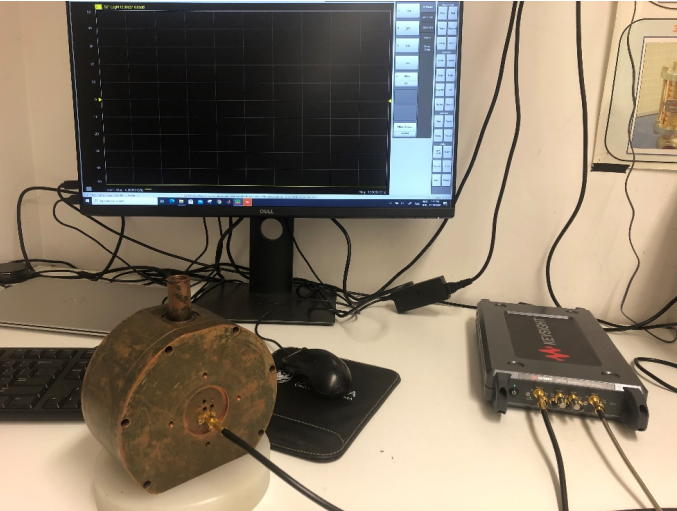
\includegraphics[width=0.28\textwidth]{4_resume}}\quad
%  \subfloat[Caption b]{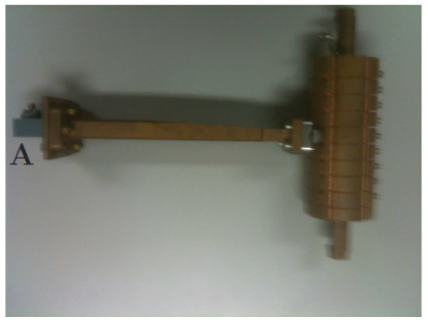
\includegraphics[width=0.28\textwidth]{3_1}}\\
%  \subfloat[Caption c]{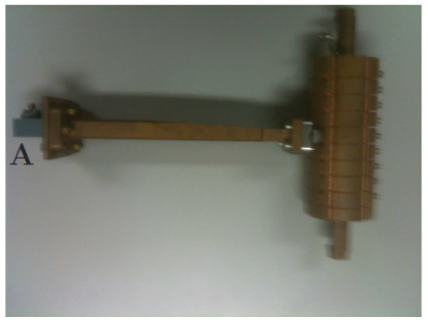
\includegraphics[width=0.28\textwidth]{3_1}}\quad
%  \subfloat[Caption d]{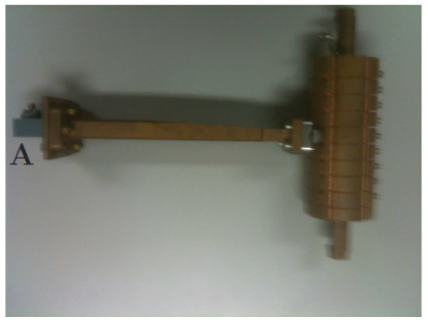
\includegraphics[width=0.28\textwidth]{3_1}}
\end{figure}
\end{frame}

\section{Appendix}
\begin{frame}[t,fragile]{Appendix (1) - Multi mode cavaty}
\begin{figure}
  \centering
  \subfloat[]{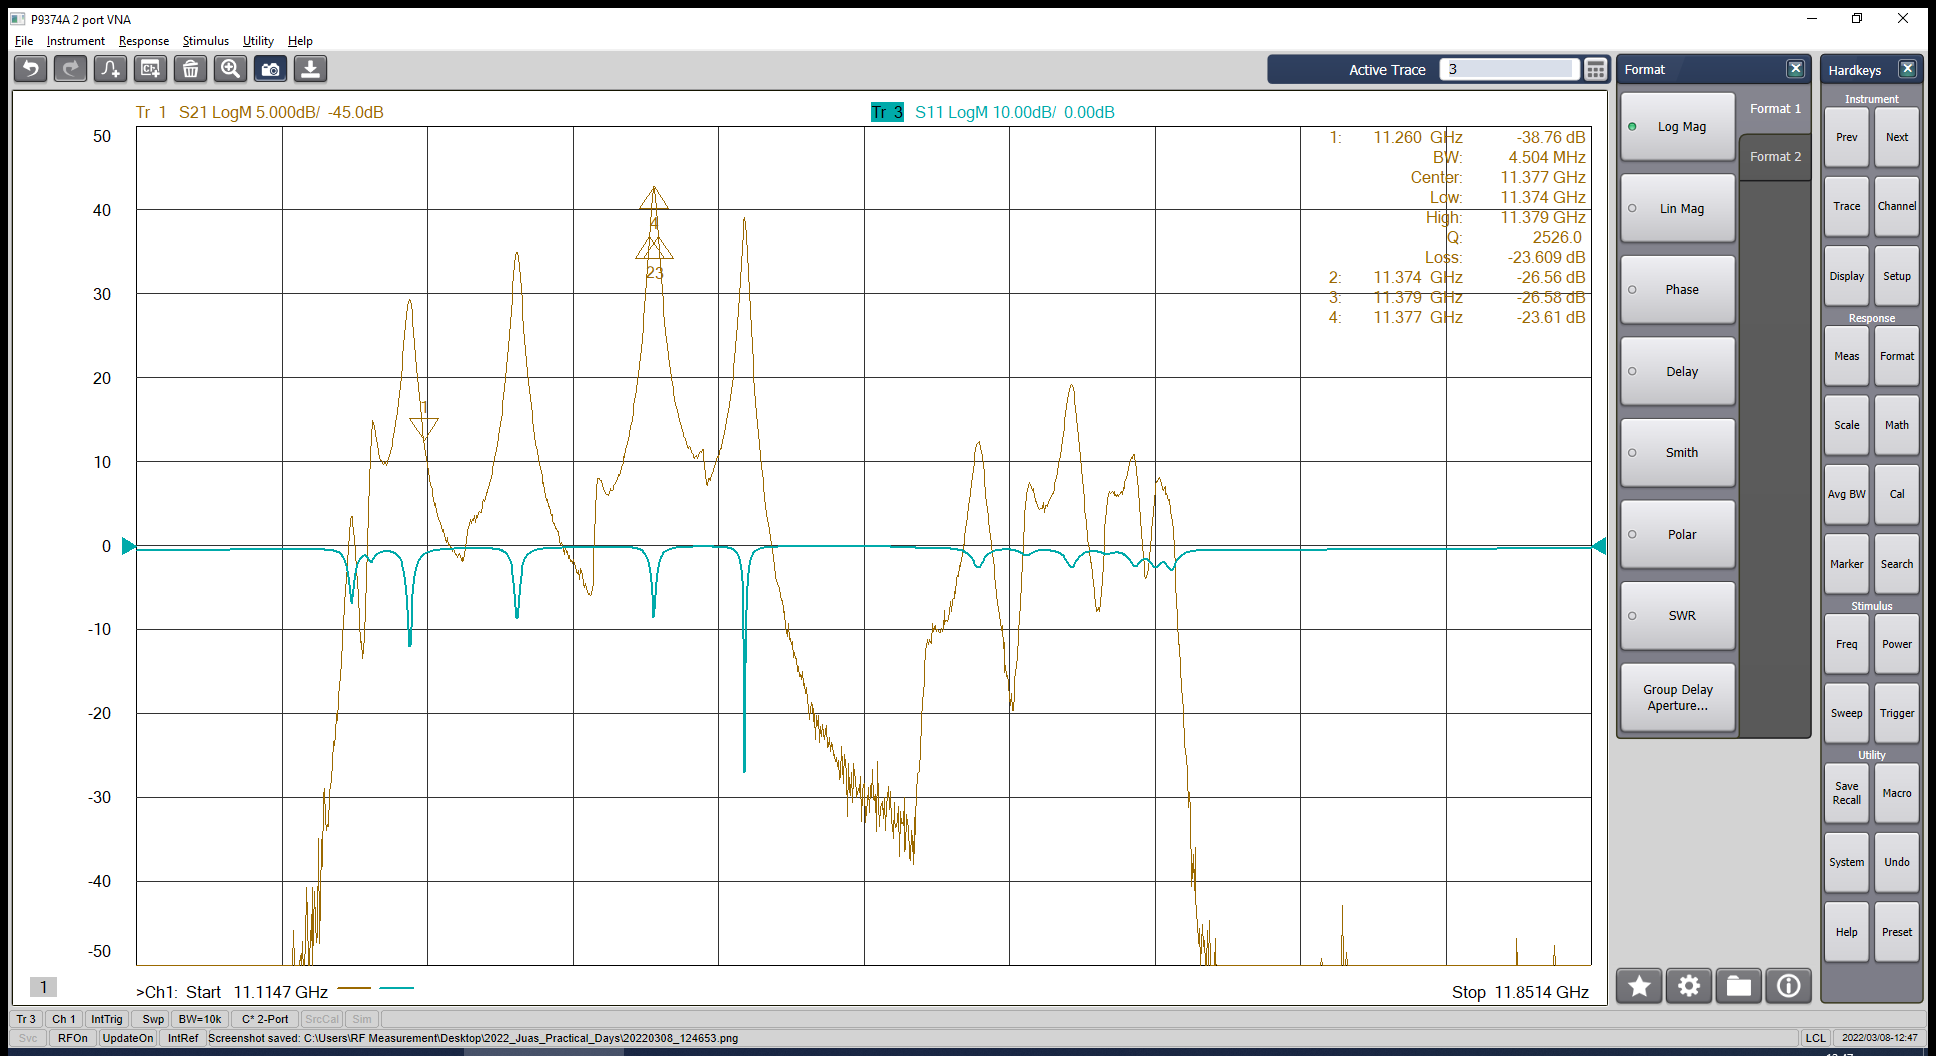
\includegraphics[width=0.45\textwidth]{5_3}}\quad
  \subfloat[]{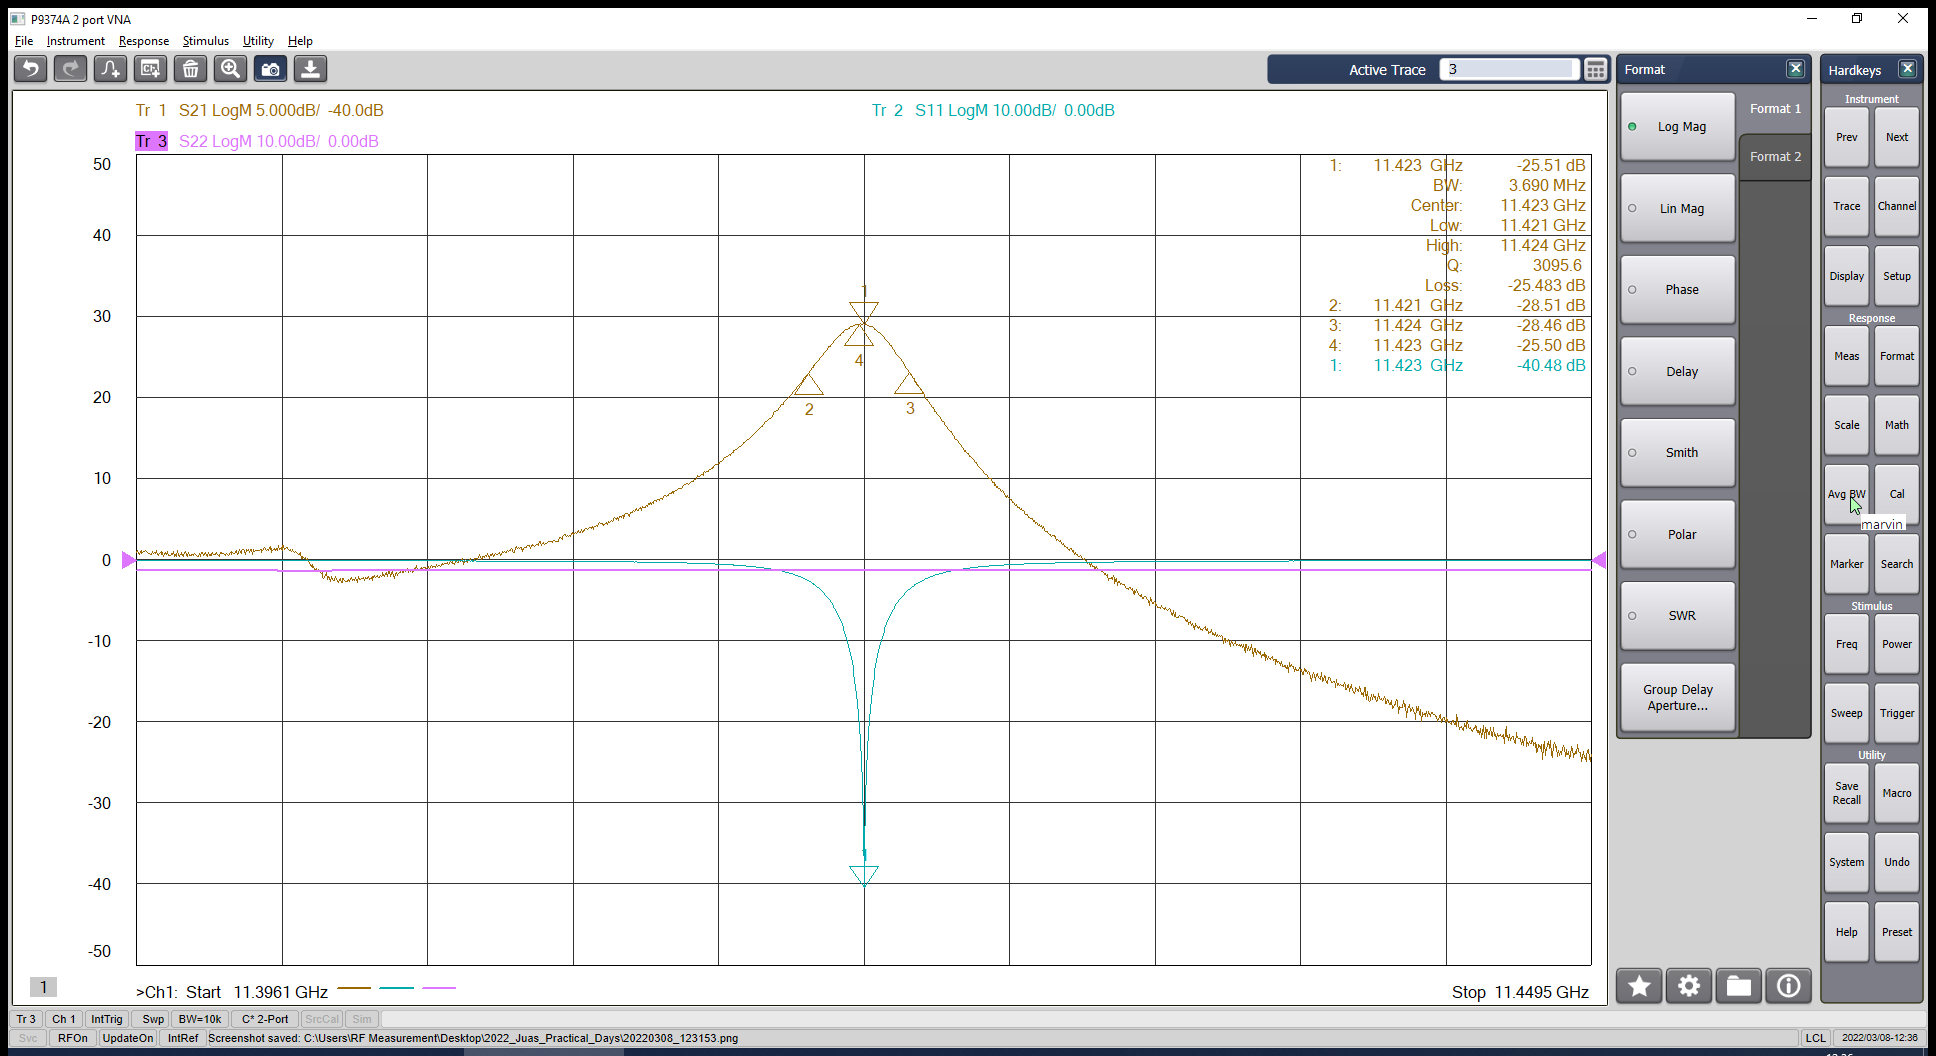
\includegraphics[width=0.45\textwidth]{5_3_2}}\\
%  \subfloat[]{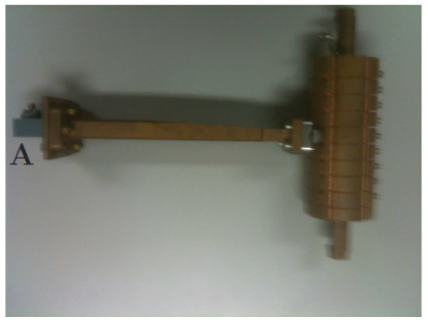
\includegraphics[width=0.28\textwidth]{3_1}}\quad
%  \subfloat[]{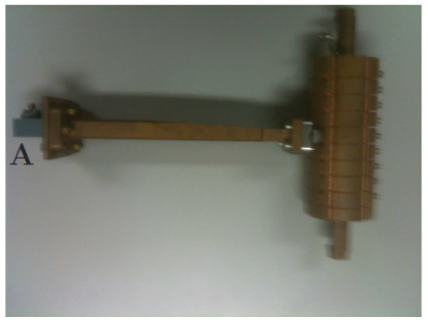
\includegraphics[width=0.28\textwidth]{3_1}}
\end{figure}
\end{frame}

\end{document}
